\subchapter{Bootloader - U-Boot}{Objectives: Set up serial
  communication, compile and install the U-Boot bootloader, use basic
  U-Boot commands, set up TFTP communication with the development
  workstation.}

As the bootloader is the first piece of software executed by a
hardware platform, the installation procedure of the bootloader is
very specific to the hardware platform. There are usually two cases:

\begin{itemize}

\item The processor offers nothing to ease the installation of the
  bootloader, in which case the JTAG has to be used to initialize
  flash storage and write the bootloader code to flash. Detailed
  knowledge of the hardware is of course required to perform these
  operations.

\item The processor offers a monitor, implemented in ROM, and through
  which access to the memories is made easier.

\end{itemize}

The IGEPv2 board, which uses the DM3730 or the OMAP3530 processors, falls into
the second category. The monitor integrated in the ROM reads the MMC/SD
card to search for a valid bootloader before looking at the internal
NAND flash for a bootloader. Therefore, by using an MMC/SD card, we can
start up a OMAP3-based board without having anything installed on it.

\section{Setup}

Go to the \code{~/felabs/sysdev/bootloader} directory. 

\section{MMC/SD card setup}

The ROM monitor can read files from a FAT filesystem on the MMC/SD
card. However, the MMC/SD card must be carefully partitionned, and the
filesystem carefully created in order to be recognized by the ROM
monitor. Here are special instructions to format an MMC/SD card
for the OMAP-based platforms.

First, connect your card reader to your workstation, with the MMC/SD
card inside. Type the \code{dmesg} command to see which device is used
by your workstation. In case the device is \code{/dev/sdb}, you will see
something like:

\begin{verbatim}
sd 3:0:0:0: [sdb] 3842048 512-byte hardware sectors: (1.96 GB/1.83 GiB)
\end{verbatim}

If your PC has an internal MMC/SD card reader, the device may also been
seen as \code{/dev/mmcblk0}, and the first partition as
\code{mmcblk0p1}. \footnote{This is not always the case with internal
MMC/SD card readers. On some PCs, such devices are behind an internal
USB bus, and thus are visible in the same way external card readers
are}. You will see that the MMC/SD card is seen in the same
way by the IGEPv2 board.

In the following instructions, we will assume that your MMC/SD card
is seen as \code{/dev/sdb} by your PC workstation.

\fbox{\begin{minipage}{\textwidth}
{\bfseries
Caution: read this carefully before proceeding. You could destroy
existing partitions on your PC!

Do not make the confusion between the device that is used by your
board to represent your MMC/SD disk (probably \code{/dev/sda}), and the device
that your workstation uses when the card reader is inserted (probably
\code{/dev/sdb}).

So, don't use the \code{/dev/sda} device to reflash your MMC disk from
your workstation. People have already destroyed their Windows
partition by making this mistake.}
\end{minipage}}

You can also run \code{cat /proc/partitions} to list all block devices
in your system. Again, make sure to distinguish the SD/MMC card from the
hard drive of your development workstation!

Type the \code{mount} command to check your currently mounted
partitions. If MMC/SD partitions are mounted, unmount them:

\begin{verbatim}
$ sudo umount /dev/sdb1
$ sudo umount /dev/sdb2
...
\end{verbatim}

Now, clear possible MMC/SD card contents remaining from previous training 
sessions:

\begin{verbatim}
$ sudo dd if=/dev/zero of=/dev/sdb bs=1M count=256
\end{verbatim}

As we explained earlier, the TI OMAP rom monitor needs special partition geometry settings
to read partition contents. The MMC/SD card must have 255 heads and 63 sectors.

Let's use the \code{cfdisk} command to create a first partition with these settings:

\code{sudo cfdisk -h 255 -s 63 /dev/sdb}

In the \code{cfdisk} interface, create a first primary partition, starting from the beginning,
with a 64 MB size, a \code{Bootable} type and a \code{0C} type (\code{W95 FAT32 (LBA)}).
Press \code{Write} when you are done.

If you used \code{fdisk} before, you should find \code{cfdisk} much more convenient!

Format this new partition in FAT32, with the \code{boot} label (name):

\begin{verbatim}
sudo mkfs.vfat -n boot -F 32 /dev/sdb1
\end{verbatim}

Then, remove and insert your card again.

Your MMC/SD card is ready to use.

\section{U-Boot setup}

Download U-Boot from the mainline igep download site:

\begin{verbatim}
wget ftp://ftp.denx.de/pub/u-boot/u-boot-2013.10.tar.bz2
tar xvf u-boot-2013.10.tar.bz2
cd u-boot-2013.10
\end{verbatim}

Then, apply the
\code{0001-arm-omap-i2c-don-t-zero-cnt-in-i2c_write.patch} patch from
this lab's \code{data} directory:

{\small
\begin{verbatim}
cat /path/to/0001-arm-omap-i2c-don-t-zero-cnt-in-i2c_write.patch | \
   patch -p1
\end{verbatim}
}

Get an understanding of its configuration and compilation steps by
reading the \code{README} file, and specifically the {\em Building the
  software} section.

Basically, you need to:

\begin{itemize}

\item set the \code{CROSS_COMPILE} environment variable;

\item run \code{make <NAME>_config}, where \code{<NAME>} is the name
  of your board as declared in the \code{boards.cfg} file. There are
  two flavors of the IGEPv2: since the RevC6 they use a NAND flash
  (\code{igep0020_nand}) and before this revision they were a OneNAND flash
  (\code{igep0020}). Note that for our platform, the configuration
  file is \code{include/configs/igep00x0.h}. Read this file to get an
  idea of how a U-Boot configuration file is written;

\item Finally, run \code{make}\footnote{You can speed up the compiling
  by using the \code{-jX} option with \code{make}, where X is the number of parallel
  jobs used for compiling. Twice the number of CPU cores is a good
  value.}, which should build U-Boot.

\end{itemize}

You can now copy the generated \code{MLO} and \code{u-boot.img} files
to the MMC card. \code{MLO} is the first stage bootloader,
\code{u-boot.img} is the second stage bootloader.

Unmount the MMC card partition.

\section{Setting up serial communication with the board}

Plug the IGEPv2 board on your computer using the provided
USB-to-serial cable. When plugged-in, a serial port should appear,
\code{/dev/ttyUSB0}.

You can also see this device appear by looking at the output of
\code{dmesg}.

To communicate with the board through the serial port, install a
serial communication program, such as \code{picocom}:

\begin{verbatim}
sudo apt-get install picocom
\end{verbatim}

You also need to make your user belong to the \code{dialout} group to be
allowed to write to the serial console:

\begin{verbatim}
sudo adduser $USER dialout
\end{verbatim}

You need to log out and in again for the group change to be effective.

Run \code{picocom -b 115200 /dev/ttyUSB0}, to start serial
communication on \code{/dev/ttyUSB0}, with a baudrate of 115200. If
you wish to exit \code{picocom}, press \code{[Ctrl][a]} followed by
\code{[Ctrl][x]}.

\section{Testing U-Boot on the MMC card}

Insert the MMC card into the IGEP board, reset the board and check
that it boots your new bootloaders. You can verify this by checking
the build dates:

\begin{verbatim}
U-Boot SPL 2013.10 (Nov 15 2013 - 14:12:51)
reading u-boot.img
reading u-boot.img


U-Boot 2013.10 (Nov 15 2013 - 14:12:51)

OMAP36XX/37XX-GP ES1.2, CPU-OPP2, L3-200MHz, Max CPU Clock 1 Ghz
IGEPv2 + LPDDR/NAND
I2C:   ready
DRAM:  512 MiB
NAND:  512 MiB
MMC:   OMAP SD/MMC: 0
*** Warning - bad CRC, using default environment

In:    serial
Out:   serial
Err:   serial
Die ID #415c00029ff80000015913d80702502a
Net:   smc911x-0
Hit any key to stop autoboot:  0 
\end{verbatim}

The message \code{reading u-boot.img} also confirms that U-Boot has
been loaded from the MMC device. You don't get it when you boot from
NAND flash (there are no files on raw flash anyway).

Interrupt the countdown to enter the U-Boot shell:
\begin{verbatim}
U-Boot #
\end{verbatim}

In U-Boot, type the \code{help} command, and explore the few commands available.

\section{Reflashing from U-boot}

We will flash U-boot and later the kernel and filesystem in NAND
flash. As far as bootloaders are concerned, the layout of the NAND
flash will look like:

\begin{center}
  \includegraphics[width=\textwidth]{labs/sysdev-u-boot/flash-map.pdf}
\end{center}

\begin{itemize}
\item Offset \code{0x0} for the first stage bootloader is dictated by
  the hardware: the ROM code of the OMAP looks for a bootloader at
  offset \code{0x0} in the NAND flash.
\item Offset \code{0x80000} for the second stage bootloader is decided
  by the first stage bootloader. This can be changed by changing the
  U-Boot configuration.
\item Offset \code{0x260000} of the U-Boot environment is also decided
  by the U-Boot configuration.
\end{itemize}

Let's first erase the whole NAND storage to remove its existing
contents. This way, we are sure that what we find in NAND comes from
our own manipulations:

\begin{verbatim}
nand erase.chip
\end{verbatim}

We are going to flash the first stage bootloader in NAND. To do so,
type the following commands:

\begin{verbatim}
mmc rescan
\end{verbatim}

This initializes the MMC interface.

\begin{verbatim}
fatload mmc 0 80000000 MLO
\end{verbatim}
This loads the file from MMC 0 partition 0 to memory at address
0x80000000.

\begin{verbatim}
nandecc hw
\end{verbatim}

This tells U-Boot to write data to NAND using the hardware ECC
algorithm, which the ROM code of the OMAP uses to load the first stage
bootloader.

\begin{verbatim}
nand erase 0 80000
\end{verbatim}

This command erases a 0x80000 byte long space of NAND flash from
offset 0\footnote{Of course, this is not needed here if you erased the
  whole NAND contents as instructed earlier. However, we prefer to
  write it here so that you don't forget next time you write anything
  to NAND.}.

\begin{verbatim}
nand write 80000000 0 80000
\end{verbatim}

This command writes data to NAND flash. The source is 0x80000000
(where we've loaded the file to store in the flash) and the
destination is offset 0 of NAND flash. The length of the copy is
0x80000 bytes, which corresponds to the space we've just erased
before. It is important to erase the flash space before trying to
write on it.

Now that the first stage has been transfered to NAND flash, you can
now do the same with U-Boot.

The storage offset of U-Boot in the NAND is 0x80000 (just after the
space reserved for the first stage bootloader) and the length is
0x1e0000.

After flashing the U-Boot image, also erase the U-boot environment
variables defined by the manufacturer or by previous users of your
board:

\begin{verbatim}
nand erase 260000 80000
\end{verbatim}

You can remove MMC card, then reset the IGEP board. You should see the
freshly flashed U-Boot starting.

You should now see the U-Boot prompt:

\begin{verbatim}
U-Boot #
\end{verbatim}

\section{Setting up Ethernet communication}

Later on, we will transfer files from the development workstation to
the board using the TFTP protocol, which works on top of an Ethernet
connection.

To start with, install and configure a TFTP server on your development
workstation, as detailed in the bootloader slides.

With a network cable, connect the Ethernet port of your board to the
one of your computer. If your computer already has a wired connection
to the network, your instructor will provide you with a USB Ethernet
adapter. A new network interface, probably \code{eth1} or \code{eth2},
should appear on your Linux system.

To configure this network interface on the workstation side, click on
the {\em Network Manager} tasklet on your desktop, and select {\em
  Edit Connections}.

\begin{center}
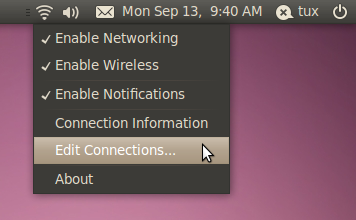
\includegraphics[width=8cm]{labs/sysdev-u-boot/network-config-1.png}
\end{center}

Select the new {\em wired network connection}:

\begin{center}
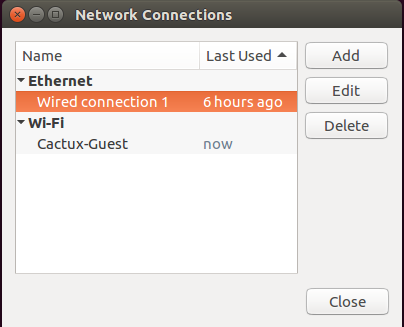
\includegraphics[width=8cm]{labs/sysdev-u-boot/network-config-2.png}
\end{center}

In the \code{IPv4 Settings} tab, press the \code{Add} button
and make the interface use a static IP
address, like \code{192.168.0.1} (of course, make sure that this
address belongs to a separate network segment from the one of the main
company network).

\begin{center}
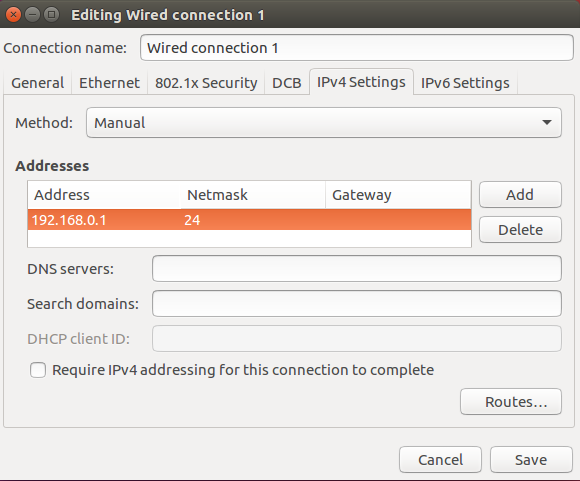
\includegraphics[width=8cm]{labs/sysdev-u-boot/network-config-3.png}
\end{center}

You can use \code{255.255.255.0} as \code{Netmask}, and leave the
\code{Gateway} field untouched (if you click on the \code{Gateway} box, you
will have to type a valid IP address, otherwise you won't be apply to
click on the \code{Apply} button).

Now, configure the network on the board in U-Boot by setting the \code{ipaddr}
and \code{serverip} environment variables:

\begin{verbatim}
setenv ipaddr 192.168.0.100
setenv serverip 192.168.0.1
\end{verbatim}

The first time you use your board, you also need to send the MAC address
in U-boot:

\begin{verbatim}
setenv ethaddr 01:02:03:04:05:06
\end{verbatim}

In case the board was previously configured in a different way, we
also turn off automatic booting after commands that can be used to
copy a kernel to RAM:

\begin{verbatim}
setenv autostart no
\end{verbatim}

To make these settings permanent, save the environment:

\begin{verbatim}
saveenv
\end{verbatim}

Now switch your board off and on again\footnote{Power cycling your
  board is needed to make your \code{ethaddr} permanent, for obscure
  reasons. If you don't, U-boot will complain that \code{ethaddr} is not
  set.}.

You can then test the TFTP connection. First, put a small text file in
the directory exported through TFTP on your development
workstation. Then, from U-Boot, do:

\begin{verbatim}
tftp 0x80000000 textfile.txt
\end{verbatim}

{\bf Caution: known issue in Ubuntu 12.04 and later}:
if this command doesn't work, you may have to stop the server
and start it again every time you boot your workstation:

\begin{verbatim}
sudo service tftpd-hpa restart
\end{verbatim}

The \code{tftp} command should have downloaded
the \code{textfile.txt} file from your development
workstation into the board's memory at location 0x80000000 (this
location is part of the board DRAM). You can verify that the download
was successful by dumping the contents of the memory:

\begin{verbatim}
md 0x80000000
\end{verbatim}

We will see in the next labs how to use U-Boot to download, flash and
boot a kernel.

\section{Rescue binaries}

If you have trouble generating binaries that work properly, or later
make a mistake that causes you to loose your \code{MLO} and
\code{u-boot.img} files, you will find working versions under
\code{data/} in the current lab directory.
